\documentclass{standalone}
\usepackage{tikz}

\begin{document}
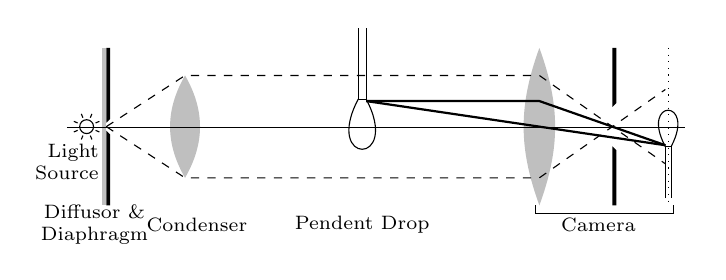
\begin{tikzpicture}[scale=0.5]
  \scriptsize % affects text nodes in this picture
  \draw (0,0) circle (5pt); % source de lumière
  \foreach \phi in { 22.5, 67.5, 112.5, 157.5 } { \draw (\phi:7pt) --
    (\phi:10pt) ; \draw (-\phi:7pt) -- (-\phi:10pt) ; } \fill[gray!50]
  (0.4,-2) rectangle (0.5,2) ; % diffuseur
  % diaphragme source
  \fill (0.5,-2) -- ++(0.1,0) -- ++(0,1.8) -- +(-0.1,0.1) -- cycle;
  \fill (0.5,2) -- ++(0.1,0) -- ++(0,-1.8) -- +(-0.1,-0.1) -- cycle;
  \fill[gray!50] (2.5,1.3) to [bend left] (2.5,-1.3) to [bend left]
  cycle; % lentille condenseur
  \draw (6.9,2.5)--(6.9,0.7)--(7.1,0.7)--(7.1,2.5); % tube
  \draw (6.9,0.7) .. controls (6,-1) and (8,-1) .. (7.1,0.7); % goutte
  \begin{scope}[yscale=-0.944/1.3] % tube et goutte image
    \draw (14.7,2.5)--(14.7,0.7)--(14.845,0.7)--(14.845,2.5); \draw
    (14.7,0.7) .. controls (14.04,-1) and (15.5,-1) .. (14.845,0.7);
  \end{scope}
  \draw[dotted] (14.77,2.0) -- +(0,-4.0); % capteur cmos
  % diaphragme camera
  \fill (13.455,2.0) -- ++(-0.1,0) -- ++(0,-1.5) -- ++(0.1,0.1) --
  cycle; \fill (13.455,-2.0) -- ++(-0.1,0) -- ++(0,1.5) --
  ++(0.1,-0.1) -- cycle;
  % lentille camera
  \fill[gray!50] (11.5,2.0) to [bend left=20] ++(0,-4) to [bend
  left=20] cycle;

  \draw[ultra thin] (-0.5,0)--(15.2,0); % axe optique
  % rayons
  \draw[dashed] (0.5,0)--(2.5,1.3)--(11.5,1.3)--(14.7,-0.944);
  \draw[dashed] (0.5,0)--(2.5,-1.3)--(11.5,-1.3)--(14.7,0.944);
  \draw[thick] (7.1,0.65)--(14.7,-0.472); % rayon objet
  \draw[thick] (7.1,0.65)--(11.5,0.65)--(14.7,-0.472);

  % legendes
  \node[align=right] at (-0.5,-0.9) {Light\\Source};
  \node[align=center] at (0.2,-2.5) {Diffusor \&\\Diaphragm}; \node at
  (2.8,-2.5) {Condenser} ; \node at (7,-2.5) {Pendent Drop};
  \draw[ultra thin] (11.4,-2.0) -- ++(0,-0.2) -- ++(3.5,0) --
  ++(0,0.2) ; \node at (13,-2.5) {Camera};
\end{tikzpicture}
\end{document}
